\documentclass{beamer}

\usetheme{Warsaw}
\usefonttheme[onlylarge]{structurebold}
\setbeamerfont*{frametitle}{size=\normalsize,series=\bfseries}
\setbeamertemplate{navigation symbols}{}

\usepackage[english]{babel}
\usepackage[utf8]{inputenc}
\usepackage{times}
\usepackage[T1]{fontenc}
\usepackage{changepage}
\usepackage[cache=false]{minted}
\usepackage{xcolor}

\definecolor{codebg}{gray}{0.9}

\title{Django Channels\\Introduction}
\author[Radoslaw Warzocha]{Radoslaw Warzocha}
%\date{I dont know the date yet}

\begin{document}

\begin{frame}
	\titlepage
\end{frame}

\section{Motivation}

\begin{frame}{Motivation}
	\begin{center}
		Django is awesome\\
		\vspace{1em}
		But it's also \textit{request} based and bound to \textit{pull/get} model\\
		\vspace{1em}
		More and more often we need to use\\
		\textit{server push} technology
	\end{center}
\end{frame}

\begin{frame}{Currently supported}
	\begin{adjustwidth}{2em}{2.5em}
	\begin{itemize}
		\item WebSockets
		\item HTTP long polling
		\item HTTP2 push
		\item Extendability to other protocols\\ (e.g. WebRTC, raw UDP, SMS)
	\end{itemize}
	\end{adjustwidth}
\end{frame}

\begin{frame}{HTTP2 utilization}
	\begin{center}
		\begin{figure}
			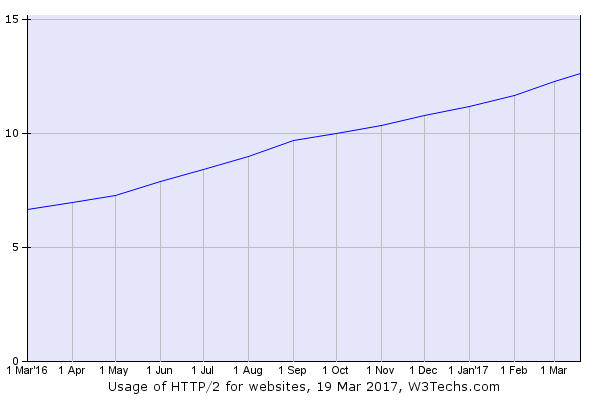
\includegraphics[scale=0.45]{ce-http2.png}
		\end{figure}
	\end{center}
\end{frame}

\section{Core concepts}

\begin{frame}{Core concepts}
	\begin{adjustwidth}{2em}{2.5em}
	\begin{itemize}
		\item Channel
			\begin{itemize}
				\item FIFO
				\item message expiry
				\item at-most-once delivery
			\end{itemize}
		\item Groups
	\end{itemize}
	\end{adjustwidth}
\end{frame}

\begin{frame}{Core concepts}
	\begin{adjustwidth}{2em}{2.5em}
	\begin{itemize}
		\item Interface/Worker servers
		\item Channels backend
		\item ASGI
		\item Consumers
		\item Routing
	\end{itemize}
	\end{adjustwidth}
\end{frame}

\section{Examples}

\begin{frame}[fragile]{Configuration}
\begin{adjustwidth}{-1.5em}{-1.5em}
	\begin{minted}
	[
	bgcolor=codebg,
	fontsize=\small,
	baselinestretch=1.2
	]
	{python}
# settings.py
CHANNEL_LAYERS = {
    "default": {
        "BACKEND": "asgiref.inmemory.ChannelLayer",
        "ROUTING": 
        	"channels_chat.routing.channel_routing",
    },
}
	\end{minted}
\end{adjustwidth}
\end{frame}

\begin{frame}[fragile]{Consumers}
\begin{adjustwidth}{-1.5em}{-1.5em}
	\begin{minted}
	[
	bgcolor=codebg,
	fontsize=\small,
	baselinestretch=1.2
	]
	{python}
from channels import Group
from .models import Message

CHAT_GROUPNAME = 'chat'

def ws_join(message):
    message.reply_channel.send({"accept": True})
    Group(CHAT_GROUPNAME).add(message.reply_channel)

def ws_leave(message):
    Group(CHAT_GROUPNAME).discard(message.reply_channel)

	\end{minted}
\end{adjustwidth}
\end{frame}

\begin{frame}[fragile]{Consumers}
\begin{adjustwidth}{-1.5em}{-1.5em}
	\begin{minted}
	[
	bgcolor=codebg,
	fontsize=\small,
	baselinestretch=1.2
	]
	{python}
def ws_message(message):
    msg = {k: message.content[k] for 
    	k in ['user', 'msg_text']}
    Message(**msg).save()
    Group(CHAT_GROUPNAME).send(msg)
	\end{minted}
\end{adjustwidth}
\end{frame}

\begin{frame}[fragile]{Routing}
\begin{adjustwidth}{-1.5em}{-1.5em}
	\begin{minted}
	[
	bgcolor=codebg,
	fontsize=\small,
	baselinestretch=1.2
	]
	{python}
from channels.routing import route
from .consumers import *

channel_routing = [
    route("websocket.connect", ws_join),
    route("websocket.receive", ws_message),
    route("websocket.disconnect", ws_leave),
]
	\end{minted}
\end{adjustwidth}
\end{frame}

\begin{frame}[fragile]{HTTP in channels}
\begin{center}
	OK, but what happens to the regular, HTTP requests?
	\pause
	No worries! That's what \textbf{\texttt{http.requests}} channel is for!
\end{center}

\begin{adjustwidth}{-1.5em}{-1.5em}
	\begin{minted}
	[
	bgcolor=codebg,
	fontsize=\small,
	baselinestretch=1.2
	]
	{python}
from django.http import HttpResponse
from channels.handler import AsgiHandler

def http_consumer(message):
    response = HttpResponse("Hello world!")
    for chunk in AsgiHandler.encode_response(response):
        message.reply_channel.send(chunk)
	\end{minted}
\end{adjustwidth}
\end{frame}

\begin{frame}[fragile]{Sessions}
\begin{adjustwidth}{-1.5em}{-1.5em}
	\begin{minted}
	[
	bgcolor=codebg,
	fontsize=\small,
	baselinestretch=1
	]
	{python}
# both cookies and `session-key`
# parameter based sessions supported
@channel_session
def ws_connect(message):
    message.reply_channel.send({"accept": True})
    room = message.content['path'].strip("/")
    message.channel_session['room'] = room
    Group("chat-%s" % room).add(message.reply_channel)

@channel_session
def ws_message(message):
    Group("chat-%s" % message.channel_session['room']).\
        send({
        "text": message['text'],
    })
	\end{minted}
\end{adjustwidth}
\end{frame}

\begin{frame}{Authentication}
	Useful decorators:
	\begin{itemize}
		\item{\textbf{\texttt{http\_session}}}
		- gives us \texttt{message.http\_session}
		\item \textbf{\texttt{http\_session\_user}} - adds \texttt{message.user}		
		\item \textbf{\texttt{channel\_session\_user\_from\_http}} -\\ all of the above \textbf{and} automatically storing user info in \textbf{both} \textit{HTTP} and \textit{channels} sessions
	\end{itemize}
\end{frame}

\subsection{Running the application}

\begin{frame}{Backends revisited}
\begin{adjustwidth}{2em}{2.5em}
	In Memmory backend is good for development, but not really suitable for production.
	
\vspace{1em}

Available backends:
	\begin{itemize}
		\item Redis
		\item Redis with Sharding
		\item IPC
		\item Write a custom one!
	\end{itemize}
\end{adjustwidth}
\end{frame}

\begin{frame}[fragile]{Running workers}
	\begin{center}
		\texttt{./manage.py runserver}\\
		will work for development "as usuall"...\\
		\pause
		by spawning both, ASGI server, and workers\\
		in one, multithreaded, process.\\
		\pause
		\vspace{1em}
		For more robust (but still local) solution, try in two different terminals:
	\end{center}
	
\begin{adjustwidth}{-1.5em}{-1.5em}
	\begin{minted}
	[
	bgcolor=codebg,
	]
	{shell}
me@terminal1$ ./manage.py runserver --no-workers
	\end{minted}
\vspace{1em}
	\begin{minted}
	[
	bgcolor=codebg,
	]
	{bash}
me@terminal2$ ./manage.py runworkers
	\end{minted}
\end{adjustwidth}
\end{frame}

\begin{frame}[fragile]{Running Workers}
We can also limit the workers to be ran on certain server:
\vspace{1em}
\begin{adjustwidth}{-1.5em}{-1.5em}
\begin{minted}
	[
	bgcolor=codebg,
	]
	{bash}
./manage.py runworkers --only-channels=http.*
\end{minted}
\vspace{1em}
\begin{minted}
	[
	bgcolor=codebg,
	]
	{bash}
./manage.py runworkers --exclude-channels=thumbnail
\end{minted}
\end{adjustwidth}
\end{frame}

\begin{frame}{Daphne}
\begin{center}
	Daphne is an Open-Source ASGI server, that comes with the Channels.\\
	\vspace{1em}
	Currently it supports:
	\begin{itemize}
		\item Websockets
		\item HTTP
		\item HTTP2 (only "normal" requests,\\ \textbf{no support for Server Push yet!} :( )
	\end{itemize}
\end{center}
\end{frame}

\begin{frame}[fragile]{Daphne}
\begin{adjustwidth}{-1.5em}{-1.5em}
	\begin{minted}
	[
	bgcolor=codebg,
	fontsize=\small,
	baselinestretch=1.2
	]
	{python}
# asgi.py
import os
from channels.asgi import get_channel_layer

os.environ.setdefault("DJANGO_SETTINGS_MODULE",
			"my_project.settings")

channel_layer = get_channel_layer()
	\end{minted}
\vspace{1em}
To run:
%\vspace{1em}
	\begin{minted}
	[
	bgcolor=codebg,
	fontsize=\small,
	baselinestretch=1.2
	]
	{bash}
$ daphne -b 0.0.0.0 -p 80 my_project.asgi:channel_layer
	\end{minted}
\end{adjustwidth}
\end{frame}

\begin{frame}
\begin{center}
	{\fontsize{30pt}{10.2}\selectfont Thank you!}\\
	\vspace{1em}
	Questions Time!
\end{center}
\end{frame}

\section{Further reading}

\begin{frame}
	\begin{description}
		\item[Django Channels] \url{https://channels.readthedocs.io/en/stable/index.html}
		\item[ASGI] \url{http://channels.readthedocs.io/en/stable/asgi.html}
		\item[Daphne] \url{https://github.com/django/daphne}
	\end{description}
\end{frame}

\end{document}
